\lecture{9}{28. Oktober 2024}{Planintegraler}
Tidligere er infinitesimalregning i flere variable behandlet i forelæsning 8, hvor der blev arbejdet med differentialregning i to varible -- dette er bl.a. brugbart indenfor maksimeringsproblemer. I dag arbejder vi med \emph{differentialregning i flere variable}s pendant -- \emph{integralregningen i flere variable}.

Planintegraler bruges til at finde volumenet under en overflade. Dette er også hvad der behandles i dag. Vi ved fra integralregningen i en variabel at
\[ 
\int_{a}^{b} f(x) \, \mathrm{d}x 
\]
indikerer arealet under funktionen $f(x)$ fra $x = a$ til $x = b$. Vi ønsker at finde et tilsvarende resultat for flere variable -- en pendant om man vil. Vi ønsker formelt set at finde volumenet under en funktion på formen $z = f(x,y)$ (Se evt. \textbf{\autoref{fig:F9_1}}). 

\begin{figure} [ht]
  \centering
  \caption{Eksempler på funktioner af flere variable}
  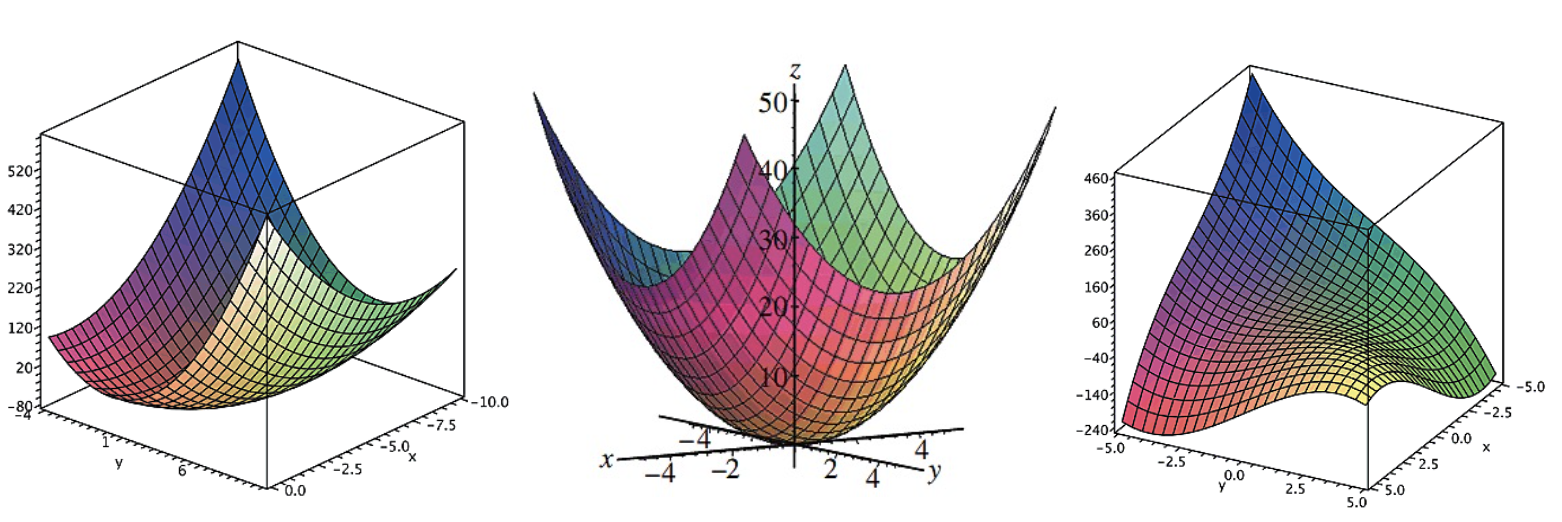
\includegraphics[width=0.5\linewidth]{./figures/F9_1.png}
  \label{fig:F9_1}
\end{figure}

\section{Indledende bemærkninger}
Hvis vi har en funktion over flere variable $f(x,y)$ kan vi integrere den ene variabel, såsom $x$, ud som
\[ 
\int_{a}^{b} f(x,y) \, \mathrm{d}x 
.\]
Her svarer det til, som var tilfældet med differentialregning i flere variable, at integrere $x$ med $y$ holdt konstant.

\begin{eks}[Simpel enkelt-integration af funktion i flere variable]
  Vi ønsker at integrere funktionen
  \[ 
  f(x,y) = x^2y^3
  ,\]
  ift. $x$. Så vi ønsker at finde
  \[ 
  \int_{0}^{1} f(x,y) \, \mathrm{d}x = \int_{0}^{1} x^2y^3 \, \mathrm{d}x 
  .\]
  Vi husker at $y$ er konstant og vi sætter derfor denne udenfor integralet
  \[ 
    y^3 \int_{0}^{1} x^2 = y^3 \left[ \frac{1}{3}x^3 \right]_0^1
  .\]
  Og vi har dermed at
  \[ 
  \int_{0}^{1} f(x,y) \, \mathrm{d}x = \frac{y^3}{3}
  .\]
\end{eks}
Vi ser fra eksemplet ovenfor at ved at vi ved at integrere $x$ ud får et udtryk der afhænger af $y$. Noget tilsvarende havde været gældende hvis vi havde integreret $y$ ud. Faktisk vil noget tilsvarende altid være gældende -- ved at integrere en variabel ud af en funktion i flere variable får du et udtryk af $n-1$ variable, hvor $n$ er antallet af variable i den oprindelige funktion.


\section{Integration over rektangler}
\begin{definition}[planintegralet]
    Lad $z = f(x,y)$ være en positiv funktion af to variable og lad $R$ betegne et rektangel
    \[ 
    a \leq x \leq b \text{og} c \leq y \leq d
    .\]
    Så har vi at 
    \[ 
    \iint_R f(x,y) \, \mathrm{d}x \, \mathrm{d}y = \int_{c}^{d} \int_{a}^{b} f(x,y) \, \mathrm{d}x \, \mathrm{d}y 
    .\]
    Dette forstås som at integrere funktionen to gange. Først integreres den ene variabel ud og dernæst integreres den anden variabel ud. Husk i øvrigt fra reglen før at hvis din funktion kun er i to variable vil planintegralet give et tal -- arealet under kurven.
\end{definition}

\begin{eks}[simpelt planintegral]
  Vi har en funktion
  \[ 
  f(x,y) = x^2y^3
  ,\]
  som skal integreres over rektanglen, $R$, defineret ved
  \[ 
  R = 0 \leq x \leq 1 \text{og} 0 \leq y \leq 2
  .\]
  Det er så at sige dette område $R$ som vi ``integrerer over''. Vi ønsker nu at udregne planintegralet af funktionen. Vi starter med at sætte afgrænsningerne ind
  \[ 
  \int_{0}^{2} \int_{0}^{1} x^2y^3 \, \mathrm{d}x \, \mathrm{d}y 
  .\]
  Først udregnes det inderste integrale givet ved
  \[ 
  \int_{0}^{1} x^2y^3 \, \mathrm{d}x 
  ,\]
  resultatet heraf er tidligere fundet til
  \[ 
  \int_{0}^{1} x^2y^3 \, \mathrm{d}x = \frac{y^3}{3}
  .\]
  Dette integreres nu over $y$-intervallet så
  \begin{align*}
    \int_{0}^{2} \frac{y^3}{3} \, \mathrm{d}y &= \frac{1}{3} \int_{0}^{2} y^3 \, \mathrm{d}y \\
    &= \frac{1}{3} \left[ \frac{y^4}{4} \right]_0^2  \\
    &= \frac{1}{3} \cdot \frac{1}{4} \cdot 2^4 \\
    &= \frac{4}{3}
  .\end{align*}
  Altså er volumenet under funktionen $x^2y^3$ i intervallet $0 \leq x \leq 1$ og $0 \leq y \leq 2$ lig 4/3.
\end{eks}

\begin{sæt}[Fubinis sætning]
  Der gælder at
  \[ 
  \int_{c}^{d} \int_{a}^{b} f(x,y) \, \mathrm{d}x \, \mathrm{d}y = \int_{a}^{b} \int_{c}^{d} f(x,y) \, \mathrm{d}y \, \mathrm{d}x 
  \]
  dvs. integrationsrækkefølgen ingen betydning har.
\end{sæt}


\section{Integration over generelle områder}
Alting bliver en smule mere kompliceret såfremt integrationsoverfladen ikke er et rektangel men et mere \emph{generelt} område. Vi har følgende definition

\begin{figure} [ht]
  \centering
  \caption{Eksempel på et type 1 og et type 2 område}
  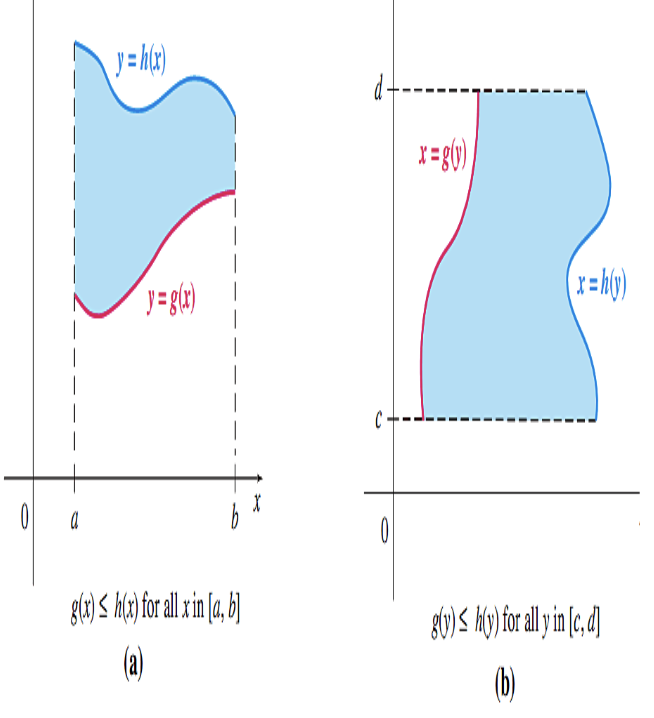
\includegraphics[width=0.4\linewidth]{./figures/F9_2.png}
  \label{fig:F9_2}
\end{figure}

\begin{definition}[Type 1 og type 2 områder]
  Vi har generelt at der eksisterer to typer af områder defineret som
  \begin{itemize}
    \item Type 1: $a \leq x \leq b$ og $g(x) \leq y \leq h(x)$
    \item Type 2: $g(y) \leq x \leq h(y)$ og $c \leq y \leq d$
  \end{itemize}
  Vi har altså for type 1 områder et overfladeintegrale på formen
  \[ 
  \iint_{R} f(x,y) \, \mathrm{d}x \, \mathrm{d}y = \int_{a}^{b} \int_{g(x)}^{h(x)} f(x,y) \, \mathrm{d}x \, \mathrm{d}y  
  .\]
  Og for type 2 områder et overfladeintegrale på formen
  \[ 
  \iint_R f(x,y) \, \mathrm{d}x \, \mathrm{d}y = \int_{g(y)}^{h(y)} \int_{c}^{d} f(x,y) \, \mathrm{d}x \, \mathrm{d}y 
  .\]
  Se evt. \autoref{fig:F9_2}.
\end{definition}

\begin{eks}[Et mere kompliceret eksempel]
  Vi ønsker at finde
  \[ 
  \iint_R \left( x^3 + 4y \right) \, \mathrm{d}y \, \mathrm{d}x 
  \]
  hvor $R$ er begrænset af
  \[ 
  y = 4x \text{og} y = x^3
  .\]
  De to funktioners skæringspunkter er i hhv. $x = 0$ og $x = 2$ og vi kan derfor tænke på det som et type 1 område og vi kan derfor opstille følgende planintegrale idet $x^3 \leq 4x$ for alle $x = [0;8]$
  \[ 
  \int_{0}^{2} \int_{x^3}^{4x} x^3 + 4y \, \mathrm{d}y \, \mathrm{d}x 
  .\]
  Vi opskriver først det inderste integral
  \[ 
    \int_{x^3}^{4x} x^3 4y \, \mathrm{d}y = [x^3y + 2y^2]_{y = x^3}^{y = 4x}
  .\]
  Vi indsætter integrationsgrænserne så vi får at
  \[
    \left( x^3 \cdot 4x + 2 \cdot (4x)^2 \right) - \left( x^3 \cdot x^3 + 2 x^{3^2} \right) = 4x^{4} + 32x^2 - 3x^{6}
  .\]
  Vi beregner nu det yderste integrale
  \begin{align*}
    \int_{0}^{2} 4x^{4} + 32x^2 - 3x^{6} \, \mathrm{d}x &= [\frac{4}{5} x^{5} + \frac{32}{3}x^3 - \frac{3}{7}x^{7}]_{x = 0}^{x = 2}  \\
    &=  56,07\ldots
  .\end{align*}
  Altså er volumenet af funktionen $f(x,y) = x^3 + 4y$ over området mellem funktionerne $y = 4x$ og $y = x^3$ lidt over 56.
\end{eks}


